\exercise

Given the undirected and weighted graph $$G = \big\{ (A, B, 2),\ (A, F, 4),\ (A,
E, 6),\ (B, C, 1),\ (B, F, 3),\ (C, D, 3),\ (C, F, 5) \big\}$$
%
\begin{enumerate}

  \item compute the MST via the Prim's algorithm by detailing the use of its
  data structures and starting from the root-node $A$.

  \item discuss the efficiency of Prim's algorithm when the graph grows in size
  (i.e. as a function of $m$ and $n$).

\end{enumerate}

\solution

\begin{enumerate}

  \item Prim's algorithm uses a prioity queue ordered by the minimum-cost edge
  incident in a node. The algorithm starts form node $A$ and performs the
  operations listed in \autoref{tab:prim}.

  \item If $n < M$ the priority queue fits in internal memory and every node
  extraction takes 0 I/Os, but the update of the priority queue needs to scan on
  disk the adjacency list, paying
  $\left\lceil\frac{\text{adj}(u)}{B}\right\rceil$ I/Os. If we sum over all the
  nodes, it is $|V| + \frac{|E|}{B}$ I/Os.

\end{enumerate}
%
\begin{figure}[t]
  \begin{subfigure}[m]{0.6\linewidth}
    \centering
    \begin{tabular}{c|c|c|c|c|c|c|c|}
      & Operation & $A$ & $B$ & $C$ & $D$ & $E$ & $F$ \\ \hline\hline
      0. & --  & $0_A$ & \infty & \infty & \infty & \infty & \infty \\ \hline
      1. & Extract $A$ & \bullet & $2_A$ & \infty & \infty & $6_A$ & $4_A$ \\ \hline
      2. & Extract $B$ & & \bullet & $1_B$ & \infty & $6_A$ & $3_B$ \\ \hline
      3. & Extract $C$ & & & \bullet & $3_C$ & $6_A$ & $3_B$ \\ \hline
      4. & Extract $D$ & & & & \bullet & $6_A$ & $3_B$ \\ \hline
      5. & Extract $F$ & & & & & $6_A$ & \bullet \\ \hline
      6. & Extract $E$ & & & & & \bullet & \\ \hline
    \end{tabular}
    \caption{}
    \label{tab:prim}
  \end{subfigure}
  %
  \begin{subfigure}[m]{0.4\linewidth}
    \centering
    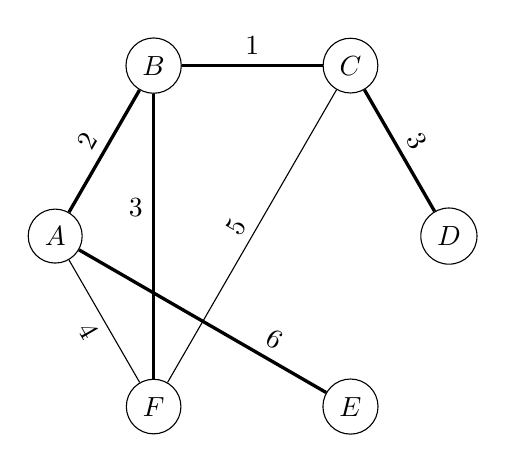
\begin{tikzpicture}
      \def \radius {2.5cm}

      \node[draw, circle] (D) at (0:\radius) {$D$};
      \node[draw, circle] (C) at (60:\radius) {$C$};
      \node[draw, circle] (B) at (120:\radius) {$B$};
      \node[draw, circle] (A) at (180:\radius) {$A$};
      \node[draw, circle] (F) at (240:\radius) {$F$};
      \node[draw, circle] (E) at (300:\radius) {$E$};

      \path (A) edge[very thick] node[sloped, above] {2} (B);
      \path (A) edge node[sloped, below] {4} (F);
      \path (A) edge[very thick] node[pos=0.75, sloped, above] {6} (E);
      \path (B) edge[very thick] node[sloped, above] {1} (C);
      \path (B) edge[very thick] node[pos=0.4, left] {3} (F);
      \path (C) edge[very thick] node[sloped, above] {3} (D);
      \path (C) edge node[sloped, above] {5} (F);
    \end{tikzpicture}
    \caption{}
    \label{fig:mst-prim}
  \end{subfigure}

  \caption{{\bf (a)} Operations computed by Prim's algorithm. Numerical values
  are expressed as $C_\pi$, where $C$ is the cost of the edges and $\pi$ their
  parent node, as stored in the priority queue. {\bf (b)} Graphical
  representation of graph $G$. Thick lines represent the final minimum spanning
  tree.}

\end{figure}
